% !TeX root = incremental_SS_Translation.tex

\chapter{Śārīrasthāna 1:  On the consideration of all beings}



\section{Literature} 

Meulenbeld offered an annotated overview of this chapter and a
bibliography of earlier scholarship to
2002 and, in his notes, citations of the parallel passages in the 
\CS.\fvolcite{IA}[243]{meul-hist}   The short account of Sāṅkhya philosophy 
offered in this chapter of the \SS\ is several times characterized as being special 
to physicians.\footnote{3.1.11 \dev{vaidyake tu} ``but in medicine\ldots''; 
3.1.13 \dev{cikitsite} ``in medicine''; 3.1.16 \dev{āyurvedaśāstreṣu} ``in the 
treatises about medicine\ldots ''; 3.1.16 \dev{sa eṣa 
karmapuruṣaścikitsādhikṛtaḥ} ``it is this agentic person that medicine is 
concerned with.''} Recent overviews of the classical theory include those of 
\textcites{ruzs-2025}[ch.\,22]{adam-2022}[\S2.4]{chat-2021}.
\citet{comb-2011} studied the specifically Ayurvedic interpretations of Indian 
philosophical ideas.

\citeauthor{solo-1974} pointed out that the description of Ahaṅkāra in the 
Māṭhara's early commentary on the \emph{Sāṅkhyakārikā} (ca.\ 1000) is 
unique in the following regard:\footcite[52, 180]{solo-1974}
\begin{quote}
    All [early Sāṅkhya commentaries]
    mention the paryāyas of ahaṃkāra, viz.\ bhūtādi, vaikṛta
    and taijasa; but all except M[āṭharavṛtti] simply state that the 16
    are produced from ahaṃkāra and enumerate them. M[āṭharavṛtti] 
    alone explains here that the five tanmātras are produced
    from bhūtādi which is tāmasa, the 11 organs are
    produced from vaikṛta which is sāttvika, while both
    are produced from taijasa which is rājasa.     
\end{quote}
Thus, the description of the evolution from Ahaṅkāra given in the \SS\ 3.1.4 
(p.\,\pageref{3.1.4}) corresponds more to that of the \textit{Māṭharavṛtti} and 
to those of the Purāṇas (Figure~\ref{fig:biardeau1981-p27}) that to other 
commentaries on the \emph{Sāṅkhyakārikā}.

\newpage

\section{Translation}

\begin{translation}
    
    \item [1] 
    
    So, now we shall explain anatomy chapter that is a reflection about all 
    beings.\footnote{The Nepalese version has nouns in apposition 
    (“-\dev{cintā} $\leftrightarrow$ \dev{śārīram}”).  The vulgate makes this a 
    single 
    karmadhāraya compound that is slightly easier to parse.} 
    
\item[3]

%The cause of all beings, called “the unmanifest,” is without a cause,
%is characterised by sattva, rajas and tamas,  has eight forms and
%is the reason for the appearance  of this whole world.

That which is called “the unmanifest” is the causeless cause of all living beings,  
having the characteristics of sattva, rajas and tamas, having eight forms, and 
being the reason for the appearance of this whole world.
    
It is the single basis of the many \se{kṣetrajña}{knowers of the
    field}, just as the ocean is to the beings who live in
water.\footnote{The Nepalese witnesses differ from the vulgate here,
    reading \dev{udakaujas} “creatures whose power is water.”  This is
    linguistically and semantically implausible. Ḍalhaṇa remarked that
    there were different interpretations of this simile in the vulgate
    version, \dev{audakānām} “creatures having watery character." Some
    thought it meant ``like rivers, lakes and other forms of water are
    supported by the ocean", while other thought it referred to living
    beings like fish and plants that are supported by the ocean." The
    emendation to \dev{udakaukas} suggested by Philipp Maas is compelling
    semantically and palaeographically.}
    
\item[3.1.4]
\label{3.1.4}
From that unmanifest, the Mahat arises, having exactly the same
properties.\footnote{In classical Sāṅkhya theory, \dev{mahat} is a
    synonym for \dev{buddhi}, ``intellect.''  In the present passage, this
    identity is not explicit; rather, it is a cosmological entity.  In the
    cosmology of the \emph{Pātañjalayogaśāstra}, it is pure being,
    \dev{sattāmātra} 2.19 \citep[85]{agas-1904}, it is also sometimes
    designated as the great \dev{ātman} ``great self'' in the sense of a
    universal being.} %
    From that Mahat, which has those same properties, arises the
    Ahaṅkāra, having exactly the same characteristics.\footnote{The
        Ahaṅkāra ``I-maker'' is the principle of individual identity.}  It
        has three aspects: \se{vaikārika}{mutable}, \se{taijasa}{fiery}
        and \se{bhūtādi}{elemental}.\footnote{\label{puraniccosmology}These 
        technical terms occur in the \emph{Sāṅkhykārikā} 22 as synonyms for 
        Ahaṅkāra \parencites[46--47]{sast-1948}[187--188]{wezl-1998}. They 
        also occur in the Purāṇic cosmogonies; \citet[27]{biar-1981} offered a 
        useful diagrammatic representation of these showing these relationships, 
        reproduced in Figure~\ref{fig:biardeau1981-p27}.}
          
            \begin{figure}
                \centering
                %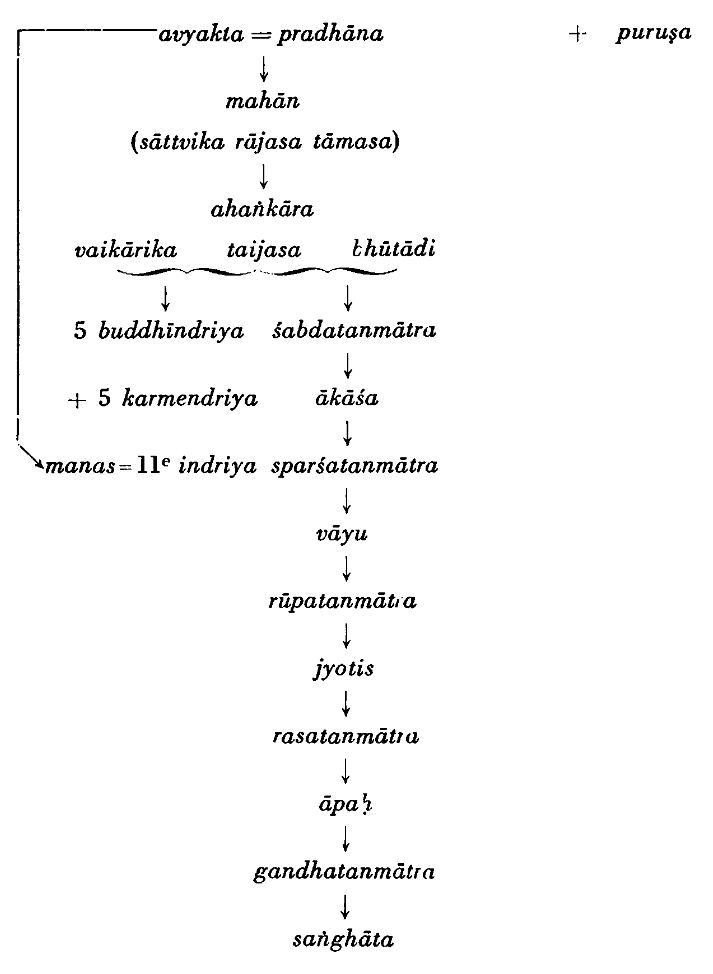
\includegraphics[height=\textheight]{chapters/media/biardeau1981-p27}
                \begin{tikzpicture}[
                  node distance=0.4cm,
                  every node/.style={font=\itshape},
                  box/.style={align=center}
                  ]
                  
                  % Top nodes
                  \node (avyakta) {avyakta = pradhāna};
                  \node[right=3cm of avyakta] (purusa) {+ \; \textit{puruṣa}};
                  
                  % Main vertical line
                  \node[below=of avyakta] (mahan) {mahān};
                  \node[below=of mahan] (gunas) {(sāttvika \; rājasa \; tāmasa)};
                  \node[below=of gunas] (ahamkara) {ahaṅkāra};
                  
                  % Threefold division with extra spacing
                  \node[below left=1cm and 2.5cm of ahamkara] (vaikarika) 
                  {vaikārika};
                  \node[below=1cm of ahamkara] (taijasa) {taijasa};
                  \node[below right=1cm and 2.5cm of ahamkara] (bhutadi) 
                  {bhūtādi};
                  
                  % Wavy brace under the three nodes
                  \draw[decorate, decoration={snake, amplitude=1mm, segment 
                      length=6mm}]
                  ([yshift=-3mm]vaikarika.south west) -- ([yshift=-3mm]bhutadi.south 
                  east);
                  
                  % From vaikārika
                  \node[below=of vaikarika] (dummy1) {};
                  \node[below=1.7cm of vaikarika] (buddhi) {5 buddhīndriya};
                  \node[below=of buddhi] (karmendriya) {+ 5 karmendriya};
                  \node[below=of karmendriya] (manas) {manas = 
                  11\textsuperscript{e} 
                      indriya};
                  
                  % From taijasa
                
                    \node[below right=1.2cm  and .5cm of taijasa] (sabda) 
                  {śabdatanmātra};
                      \node[above=of sabda] (dummy2) {};
                  \node[below=of sabda] (akasa) {ākāśa};
                  \node[below=of akasa] (sparsa) {sparśatanmātra};
                  \node[below=of sparsa] (vayu) {vāyu};
                  \node[below=of vayu] (rupa) {rūpatanmātra};
                  \node[below=of rupa] (jyotis) {jyotis};
                  \node[below=of jyotis] (rasa) {rasatanmātra};
                  \node[below=of rasa] (apas) {āpaḥ};
                  \node[below=of apas] (gandha) {gandhatanmātra};
                  \node[below=of gandha] (sanghata) {saṅghāta};
                  
                  % Connections
                  \draw[->] (avyakta) -- (mahan);
                  \draw[->] (mahan) -- (gunas);
                  \draw[->] (gunas) -- (ahamkara);
                  
                  % Branches
%                  \draw[->] (ahamkara) -- (vaikarika);
%                  \draw[->] (ahamkara) -- (taijasa);
%                  \draw[->] (ahamkara) -- (bhutadi);
                  
                  % Left branch
                  \draw[->] (dummy1) -- (buddhi);
                  \draw[->] (buddhi) -- (karmendriya);
                  \draw[->] (karmendriya) -- (manas);
                  
                  % Diagonal slanted connection back into middle branch
                  %\draw[->] (manas.east) .. controls +(3,0) and +(-3,0) .. 
                  %(sparsa.west);
                  
                  % Middle branch
                  \draw[->] (dummy2) -- (sabda);
                  \draw[->] (sabda) -- (akasa);
                  \draw[->] (akasa) -- (sparsa);
                  \draw[->] (sparsa) -- (vayu);
                  \draw[->] (vayu) -- (rupa);
                  \draw[->] (rupa) -- (jyotis);
                  \draw[->] (jyotis) -- (rasa);
                  \draw[->] (rasa) -- (apas);
                  \draw[->] (apas) -- (gandha);
                  \draw[->] (gandha) -- (sanghata);
                  
              \end{tikzpicture}
              
                \caption{Levels of original creation as presented in the following 
                Purāṇas: \emph{Vāyupurāṇa}, \emph{Brahmāṇḍapurāṇa}, 
                \emph{Viṣṇupurāṇa}, \emph{Mārkaṇḍeyapurāṇa}, 
                and \emph{Kūrmapurāṇa}, \citep[after][27]{biar-1981}. 
                See footnote \ref{puraniccosmology}}
                \label{fig:biardeau1981-p27}
            \end{figure}
            
          
            
            
            From that mutable Ahaṅkāra the 
            eleven \se{indriya}{faculties} arise, with the very same
            characteristics. It is as follows: ear, skin, eye, tongue, nose,
            speech, hand, genitals, anus, feet and mind.  Amongst these, the first 
            five are the faculties of \se{buddhi}{cognition}; the next five are the 
            faculties of \se{karma}{action}.  The mind has properties of both.
            
            From the Ahaṅkāra as \se{bhūtādi}{starting point for the
    elements}, arise the five \se{tanmātra}{bare entities},
with exactly the same characteristics.\footnote{Earlier,
    the Ahaṅkāra was said to have three aspects, so we would
    here expect a description of the \se{taijasa}{fiery}
    aspect.  But the Nepalese version goes straight to the
    \se{bhūtādi}{elemental} aspect.  The vulgate text inserts
    the fiery aspect alongside the elemental as if it were
    similar in all respects (\dev{taijasasahāya}).}  It is as
    follows: bare sound, bare touch, bare form, bare taste,
    bare smell.\footnote{Or, ``the essence of sound,'' etc.}
    
    From these \se{bhūta}{elements} come space, air, fire, water and earth; 
    from these come sound, touch, form, taste and smell, with the same 
    distinctions.  In this way these twenty-four \sepl{tattva}{principle} have 
    been explained. 
            
\item[5]    

In this context, sound and so on are the objects of the \se{indriya}{faculties} of 
cognition.  Amongst the faculties of action, they are: speaking, holding, 
enjoyment, excretion and walking respectively.  

\item[6]

The eight \se{prakṛti}{productive principles} are 
the \se{avyakta}{unmanifest},
\se{mahān}{The Great}, 
the \se{ahaṅkāra}{I-principle}, 
and the five \se{tanmātra}{fine elements}.
The rest are the sixteen \se{vikāra}{modifications}.
    
\item[7]   

Each and every one of them has a sovereign with respect to their
domain.  There is their own \se{adhyātmika}{personal aspect} and the
\se{adhidaiva}{divine aspect}. Thus, \\
\begin{center}
\begin{tabular}{ll}
\toprule
\emph{Divine} & \emph{Personal}\\
\midrule
    Brahmā & of Buddhi,\\
Īśvara &of ahaṃkāra,\\
the moon &of mind,\\
the ear &of the directions,\\
wind &of the skin,\\
the sun & of the eyes,\\
the waters &of the tongue,\\
the earth &of the nose,\\
fire &of the voice,\\
Indra & of the hands,\\
Viṣṇu &of the feet,\\
Mitra & of the anus,\\
and Prajāpati &of the genitals7.\\
\bottomrule
\end{tabular}
\end{center}
%Brahmā of Buddhi,
%Īśvara of ahaṃkāra,
%the moon of mind,
%the ear of the directions,
%wind of the skin,
%the sun for the eyes,
%the waters for the tongue,
%the earth for the nose,
%fire for the voice,
%Indra for the hands,
%Viṣṇu for the feet,
%Mitra for the anus,
%and Prajāpati for the penis.


% everything except the mahābhūtas and tanmātras - CB







\end{translation}
